% !TeX document-id = {35195650-eebd-4fc9-a058-5836dd2c9fdc}
%!TEX program = PdfLatex
\documentclass[newPxFont,sthlmFooter]{beamer}
\usetheme{sthlm}


%-=-=-=-=-=-=-=-=-=-=-=-=-=-=-=-=-=-=-=-=-=-=-=-=
%        LOADING PACKAGES
%-=-=-=-=-=-=-=-=-=-=-=-=-=-=-=-=-=-=-=-=-=-=-=-=
\usepackage[UTF8,space]{ctex}
% 
% Note: If you use ctex package to support chinese, please go to ctex.sty to comment the line 
% "\ctex_hypersetup:n { colorlinks = ture }"  or set "colorlinks = false". Else you will see an ugly
% toc, too ugly!!!   2015/12/12  by hongxing xia (xiahongxing@gmail.com)


\usepackage{chronology}

\renewcommand{\event}[3][e]{%
  \pgfmathsetlength\xstop{(#2-\theyearstart)*\unit}%
  \ifx #1e%
    \draw[fill=black,draw=none,opacity=0.5]%
      (\xstop, 0) circle (.2\unit)%
      node[opacity=1,rotate=45,right=.2\unit] {#3};%
  \else%
    \pgfmathsetlength\xstart{(#1-\theyearstart)*\unit}%
    \draw[fill=black,draw=none,opacity=0.5,rounded corners=.1\unit]%
      (\xstart,-.1\unit) rectangle%
      node[opacity=1,rotate=45,right=.2\unit] {#3} (\xstop,.1\unit);%
  \fi}%

%-=-=-=-=-=-=-=-=-=-=-=-=-=-=-=-=-=-=-=-=-=-=-=-=
%        BEAMER OPTIONS
%-=-=-=-=-=-=-=-=-=-=-=-=-=-=-=-=-=-=-=-=-=-=-=-=

%\setbeameroption{show notes}

%-=-=-=-=-=-=-=-=-=-=-=-=-=-=-=-=-=-=-=-=-=-=-=-=
%
%	PRESENTATION INFORMATION
%
%-=-=-=-=-=-=-=-=-=-=-=-=-=-=-=-=-=-=-=-=-=-=-=-=

\title{手写数字识别}
\subtitle{Handwritten Digits Recognition}
%\date{\small{\jobname}}
%\date{\today}

\author{\textbf{指导老师:覃义}}
\institute{\textbf{唐呈俊 刘宇豪 黄增玉 金梦雨}}

\date{\today}

%\institute{ 数学与计算科学学院 }

\hypersetup{
pdfauthor = {},
pdfsubject = {},
pdfkeywords = {},
pdfmoddate= {D:\pdfdate},
pdfcreator = {}
}

\begin{document}

%-=-=-=-=-=-=-=-=-=-=-=-=-=-=-=-=-=-=-=-=-=-=-=-=
%
%	TITLE PAGE
%
%-=-=-=-=-=-=-=-=-=-=-=-=-=-=-=-=-=-=-=-=-=-=-=-=

\maketitle

%\begin{frame}[plain]
%	\titlepage
%\end{frame}

%-=-=-=-=-=-=-=-=-=-=-=-=-=-=-=-=-=-=-=-=-=-=-=-=
%
%	TABLE OF CONTENTS: OVERVIEW
%
%-=-=-=-=-=-=-=-=-=-=-=-=-=-=-=-=-=-=-=-=-=-=-=-=

\section*{手写数字识别}

%-=-=-=-=-=-=-=-=-=-=-=-=-=-=-=-=-=-=-=-=-=-=-=-=
%	FRAME:
%-=-=-=-=-=-=-=-=-=-=-=-=-=-=-=-=-=-=-=-=-=-=-=-=

\begin{frame}[c]{MNIST数据集}

\begin{block}{MNIST是一个手写数字数据集:}
	其中包含60,000个示例的训练集以及10,000个示例的测试集。 它是NIST提供的更大集合的一个子集。 这些数字已经进行了尺寸标准化并以固定尺寸的图像为中心。
\end{block}

\end{frame}

\begin{frame}[c]{Softmax回归模型}

\begin{block}{Softmax回归模型是logistic回归模型在多分类问题上的推广:}
	在多分类问题中,类标签 $y$ 可以取两个以上的值。Softmax回归模型对于MNIST手写数字分类问题是很有用的。
\end{block}
\begin{align*}
h_\theta(x^{(i)}) =
\begin{bmatrix}
p(y^{(i)} = 1 | x^{(i)}; \theta) \\
p(y^{(i)} = 2 | x^{(i)}; \theta) \\
\vdots \\
p(y^{(i)} = k | x^{(i)}; \theta)
\end{bmatrix}
=
\frac{1}{ \sum_{j=1}^{k}{e^{ \theta_j^T x^{(i)} }} }
\begin{bmatrix}
e^{ \theta_1^T x^{(i)} } \\
e^{ \theta_2^T x^{(i)} } \\
\vdots \\
e^{ \theta_k^T x^{(i)} } \\
\end{bmatrix}
\end{align*}

\end{frame}

\begin{frame}[c]{Softmax 回归 vs. k 个二元分类器}

\begin{block}{使用 softmax 分类器,还是使用 logistic 回归算法建立 k 个独立的二元分类器:}
	这一选择取决于你的类别之间是否互斥,在本次手写数字识别分类的任务中,我们一个图像不可能对应多个数字,所以说我们的手写数字识别是不可能出现同一个数字属于不同的数据集的情况的,所以说我们选择了softmax分类器。
\end{block}

\end{frame}

\begin{frame}[c]{梯度下降法}

\begin{block}{梯度下降(SG):}
	在求解机器学习算法的模型参数,即无约束优化问题时,梯度下降(Gradient Descent)是最常采用的方法之一。
\end{block}

\[\gamma_{n} = \frac{(\mathbf x_{n} - \mathbf x_{n-1})^T[\nabla F(\mathbf x_{n}) - \nabla F(\mathbf x_{n-1})]}{||\nabla F(\mathbf x_{n}) - \nabla F(\mathbf x_{n-1})||^2}\]

\end{frame}

\begin{frame}[c]{TensorFlow}

\begin{block}{TensorFlow是一个用于数值计算的开源软件库:}
TensorFlow™ 是一个采用数据流图(data flow graphs),用于数值计算的开源软件库。节点(Nodes)在图中表示数学操作,图中的线(edges)则表示在节点间相互联系的多维数据数组,即张量(tensor)。它灵活的架构让你可以在多种平台上展开计算,例如台式计算机中的一个或多个CPU(或GPU),服务器,移动设备等等。TensorFlow 最初由Google大脑小组(隶属于Google机器智能研究机构)的研究员和工程师们开发出来,用于机器学习和深度神经网络方面的研究,但这个系统的通用性使其也可广泛用于其他计算领域。
\end{block}

\end{frame}

\begin{frame}{程序流程图}

\begin{figure}
	\centering
	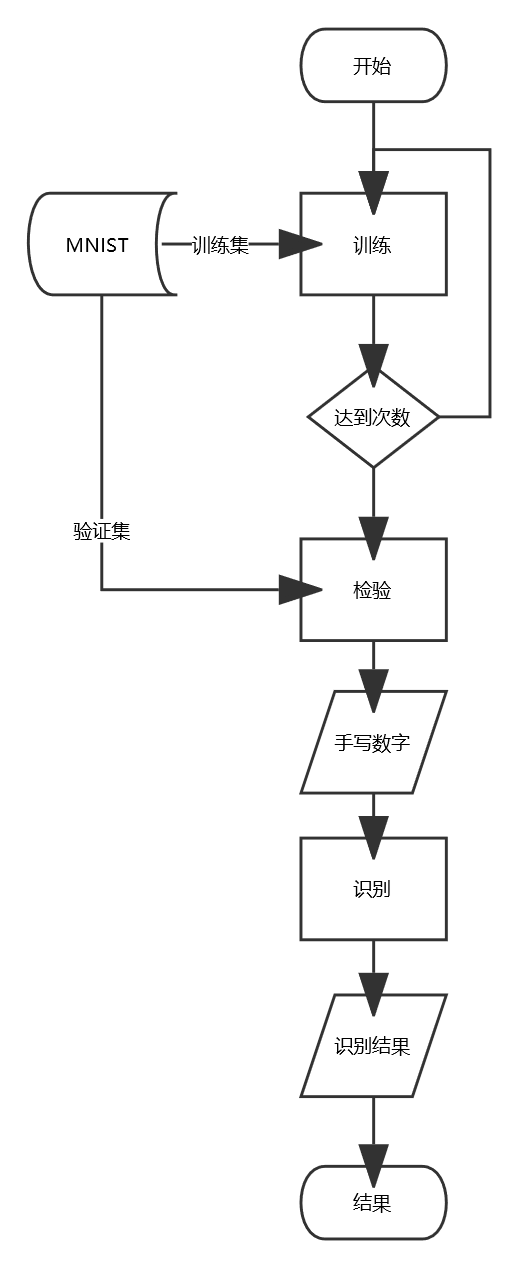
\includegraphics[height=0.7\textheight]{screenshot001}
	\caption{程序流程图}
	\label{fig:screenshot001}
\end{figure}

\end{frame}

\begin{frame}{程序运行图}

\begin{figure}
	\centering
	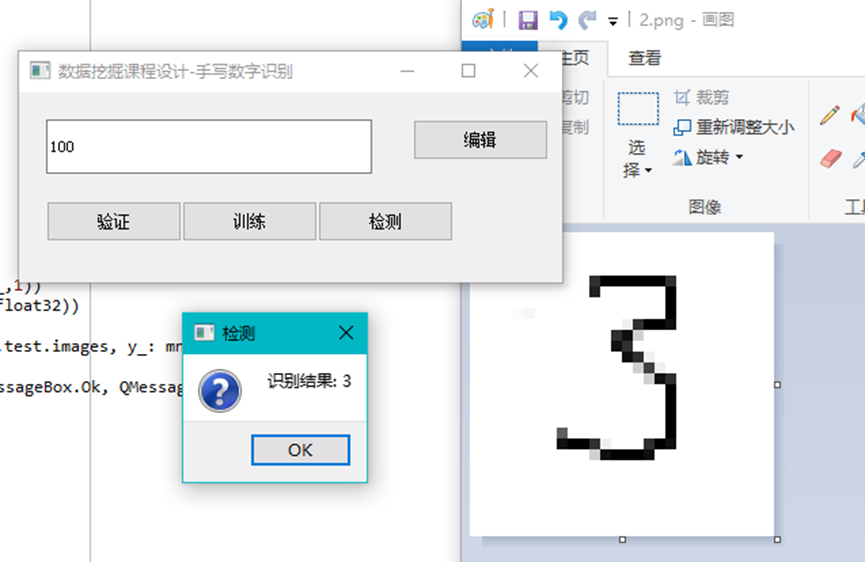
\includegraphics[width=0.7\linewidth]{screenshot002}
	\caption{程序运行图1}
	\label{fig:screenshot002}
\end{figure}

\end{frame}

\begin{frame}{程序运行图}

\begin{figure}
	\centering
	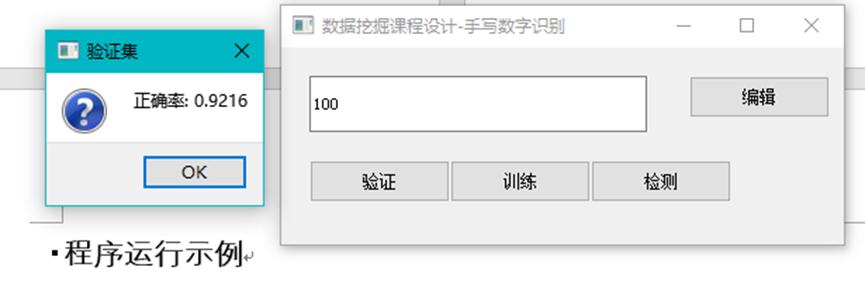
\includegraphics[width=0.7\linewidth]{screenshot003}
	\caption{程序运行图2}
	\label{fig:screenshot003}
\end{figure}

\end{frame}

\begin{frame}{参考文献}

[1] Yann LeCun. THE MNIST DATABASE
of handwritten digits [EB/OL]. http://yann.lecun.com/exdb/mnist/

[2]Google Inc. Tensor Flow[CP]. http://www.tensorflow.org/

[3] Andrew Ng. UFLDL Tutorial [DB/CD]. Stanford University,2012


\end{frame}

\end{document}
